\documentclass[a4paper]{article}

\usepackage[spanish]{babel}
\usepackage{graphicx}
\usepackage{amsmath, amssymb}
\usepackage[margin=2cm]{geometry}
\usepackage{fancyhdr}
\usepackage{enumerate}
\usepackage[shortlabels]{enumitem}
\usepackage{parskip}
\usepackage[most]{tcolorbox}
\usepackage[hidelinks]{hyperref}
\usepackage{float}


% cabecera
\pagestyle{fancy}
\fancyhead[l]{Daniel Soto}
\fancyhead[c]{Problemas de Astronomía \#5}
\fancyhead[r]{\today}
\fancyfoot[c]{\thepage}
\renewcommand{\headrulewidth}{0.2pt} % linea horizontal

%% Definicion de comandos para formato de unidades fisicas %%
\newcommand{\m}{\text{m}}
\newcommand{\cm}{\text{cm}}
\newcommand{\km}{\text{km}}
\newcommand{\s}{\text{s}}
\newcommand{\N}{\text{N}}
\newcommand{\g}{\text{g}}
\newcommand{\kg}{\text{kg}}
\newcommand{\Msolar}{\text{M}_\odot}
\newcommand{\Mterrestre}{\text{\text{M}_\oplus}}
\newcommand{\AU}{\text{AU}}
\newcommand{\ly}{\text{ly}}
\newcommand{\nT}{\text{nT}}
\newcommand{\GeV}{\text{GeV}}
\newcommand{\atomscm}{\text{atoms/cm}^3}

\newcounter{problema}

\newtcolorbox[use counter=problema]{problema}[1][]{%
    colback=gray!15,
    colframe=gray!60,
    fonttitle=\bfseries,
    title={Problema~\theproblema:},
    boxrule=0.5mm,
    arc=3mm,
    boxsep=5pt,
    left=8pt,
    right=8pt,
    top=6pt,
    bottom=6pt,
    #1
}


\begin{document}

\begin{problema}
Un campo magnético es más complicado en forma que un campo gravitacional porque los campos magnéticos tienen una propiedad llamada \textit{polaridad}. 
Todos los imanes tienen un polo magnético Norte y Sur, y dependiendo de dónde te encuentres en el espacio cerca de un imán, 
la fuerza que sentirás será diferente a la de la gravedad. 

	\begin{figure}[H]
    		\centering
    		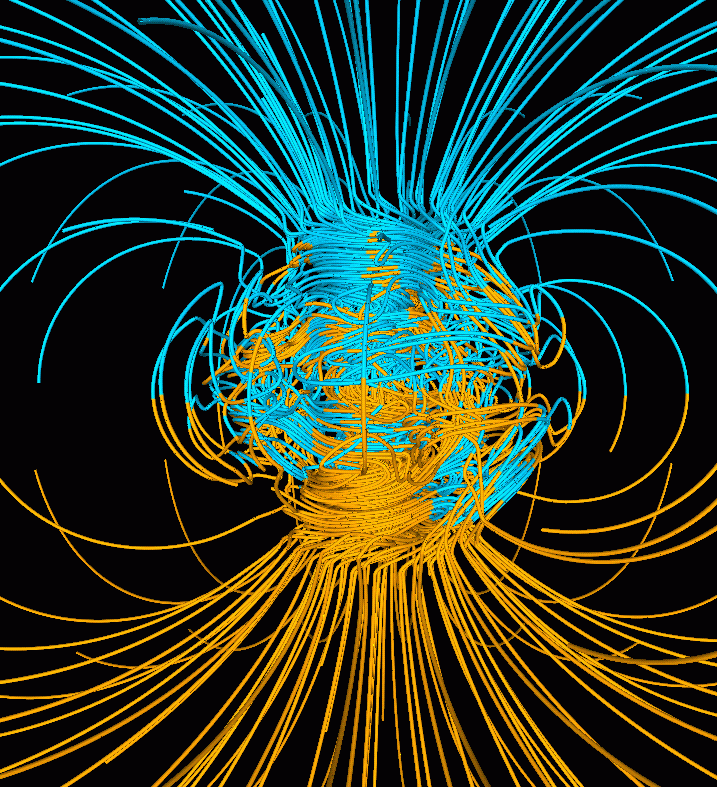
\includegraphics[width=0.5\textwidth]{earthMagneticField.png}
    		\caption{Simulacion campo magnético de la tierra}
    		\label{fig:1}
	\end{figure}

La intensidad del campo magnético a lo largo de cada una de las tres direcciones en el espacio $(x, y, z)$ viene dada por las siguientes fórmulas:

\begin{align*}
B_x &= 3xz\frac{M}{r^5} \\
B_y &= 3yz\frac{M}{r^5} \\
B_z &= \left(3z^2-r^2\right)\frac{M}{r^5}
\end{align*}

Las variables $(x, y, z)$ representan la distancia a un punto en el espacio en términos del radio de la Tierra. Por ejemplo, $x = 2.4$ significa una distancia física de 2.4 veces el radio de la Tierra o $2.4 \times 6 378 \km \approx 15 000 \km$. Cualquier punto en el espacio cerca de la Tierra puede describirse mediante su dirección $(x, y, z)$. La variable $r$ es la distancia desde el punto en $(x, y, z)$ hasta el centro de la Tierra en unidades del radio de la Tierra. $M$ es una constante igual a $31 000$ nanoTeslas ($\nT$).

La fórmula para las tres cantidades $(B_x, B_y, B_z)$ proporciona sus intensidades a lo largo de cada una de las tres direcciones en el espacio, en unidades de $\nT$, una medida de la intensidad magnética.

\vspace{5mm}
\begin{enumerate}
	\item Evalúe estas tres ecuaciones en la órbita de satélites de comunicaciones para el caso donde $(x, y, z) = (7, 0, 0)$ y $r=7$
	\item Evalúe estas tres ecuaciones en los Cinturones de Van Allen para el caso donde $(x, y, z)=(0.38, 0.19, 1.73)$ y $r=3$
	\item Evalúe estas tres ecuaciones a la distancia de la Luna para el caso donde $(x, y, z) = (0, 48, 36)$ y $r=60$
	\item Utilice el Teorema de Pitágoras en tres dimensiones para determinar la magnitud absoluta del campo magnético de la Tierra para cada uno de los problemas 1, 2 y 3.
\end{enumerate}

\end{problema}
[1.2.5] \cite{algebra2}

\begin{problema}
\textbf{El Boson de Higgs:} Durante más de 30 años, los físicos buscaron signos de un nuevo tipo de partícula elemental. Actualmente conocemos electrones, protones, neutrones y muchas otras partículas.

El bosón de Higgs es único porque es la única partícula del Modelo Estándar que otorga masa a las demás partículas fundamentales a través de su interacción con el campo de Higgs.

En 2012, su existencia fue confirmada experimentalmente en el Gran Colisionador de Hadrones (LHC) del CERN: aunque no se observa directamente, la lluvia de rastros provenientes del centro de la colisión de dos protones permitió identificar su presencia.

	\begin{figure}[H]
    		\centering
    		
\includegraphics[width=0.5\textwidth]{Higgs.png}
    		\caption{Descubrimiento del bosón de Higgs en CMS (CERN). El exceso de eventos en $m_{\gamma\gamma} \approx 125 \GeV$ confirma su existencia a través de su desintegración en dos fotones.}
    		\label{fig:2}
	\end{figure}

Antes de su descubrimiento, diversos experimentos habían impuesto restricciones sobre el rango probable de su masa:


\begin{itemize}
	\item Los experimentos del acelerador Tevatrón de Fermilab indicaban que debía tener una masa mayor que $170 \GeV$ o menor que $160 \GeV$
	\item El acelerador LEP de CERN concluyó, tras años de búsqueda, que el bosón de Higgs debía tener una masa mayor que $115 \GeV$
	\item Además, cálculos basados en el Modelo Estándar (la teoría que describe las interacciones de las partículas elementales) establecieron límites teóricos: 
	la masa del bosón de Higgs no podía superar los $190 \GeV$, y debía estar entre $80 \GeV$ y $200 \GeV$, según distintos supuestos. 
\end{itemize} 

\vspace{5mm}
\begin{enumerate}
	\item A partir de todas estas restricciones previas al descubrimiento, ¿cuál era la intersección de valores de masa posibles para el bosón de Higgs que resultaba consistente con todas ellas?
	\item La masa equivalente a $100 \GeV$ es $1.7\times 10^{-25} \kg$. ¿Cuál es el rango de masas para el bosón de Higgs?
\end{enumerate}

\end{problema}
[1.6.3]\cite{algebra2}


\begin{problema}
\textbf{Colapso Gravitacional:} Las nubes de gas en el espacio interestelar no pueden permanecer como están durante mucho tiempo, ya que la gravedad de su propia masa las hace colapsar bajo su propio peso. La fórmula que relaciona el tiempo de colapso, $T$, con la densidad de la nube de gas, $N$, es:

$$T = \frac{2\times 10^6}{\sqrt{N}}$$

donde $T$ es el tiempo en años y $N$ es la densidad de la nube de gas dada en átomos por centímetro cúbico.

	\begin{figure}[H]
    		\centering
    		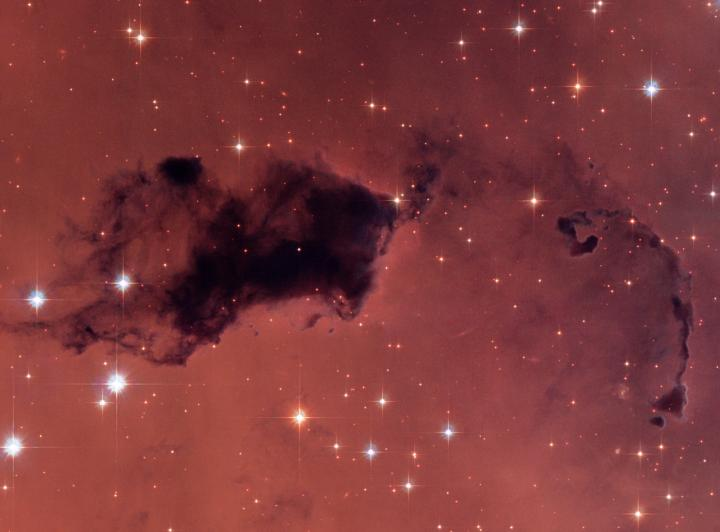
\includegraphics[width=0.5\textwidth]{BokGlobule.jpg}
		\caption{Nebulosa Pacman: NGC 281}
		\label{fig:3}
	\end{figure}
\vspace{5mm}
\begin{enumerate}
	\item Una típica nube oscura tipo \textit{Bok Globule}, con un diámetro de un año luz y que contiene aproximadamente $100$ veces la masa de nuestro Sol en gas interestelar, tiene una densidad de unos $4000 \atomscm$. 
	¿Cuál es su tiempo estimado de colapso en años?
	\item La Vía Láctea se formó originalmente a partir de una nube de gas con una densidad promedio que pudo haber sido de unos $2 \atomscm$ . ¿Cuánto tiempo tardó, aproximadamente en colapsar la nube de la Vía Láctea?
\end{enumerate}

\end{problema}
[5.3.2]\cite{algebra2}

\bibliographystyle{plainurl}
\bibliography{bibliografia} % Nombre del .bib

\end{document}
